\section{Discussion and Conclusions}

\subsection{Discuss and compare the different solution methods for the test problem used (Van der Pol and CSTR).}
We've already commented out the results of each individual method in its corresponding part. We've also compared them indirectly when discussing each particular solution. This project's findings agree with what is stated in the literature: explicit methods have problems of stability when applied to stiff ODE systems and implicit methods can be used to overcome these problems. However, solving a non-linear system of equations is required in the internal steps of implicit methods, usually solved by calling an iterative method which increases the number of function calls, creating an overhead. Thus, implicit methods are only useful when working in stiff problems with really low tolerances, where we are interested in having a very precise solution.

During the project we've looked at different Explicit methods (Explicit Euler, classical Runge-Kutta and Dormand-Prince 5(4)) and we've seen how the convergence of the solution gets better as we chose methods of higher orded. However, all these methods perform poorly when applied to stiff problems so, we tried two different implicit architectures, Implicit Euler and Explicit Simply-Diagonally Implicit Runge-Kutta 2(3) method. Both achieve overall good performance when working with stiff problems. However, the magic of the ESDIRK23 is that it manages to also keep the computational cost pretty low for non-stiff problems.

In this chapter, we are interested in the performance of the models. In order to achieve this, we'll take a look at how the different stats of every model evolve through different tolerances when applied to each particular problem. The results are shown in the following figures.

The first realisation we can make is that the ODE solvers from Matlab achieve very good performance in the Van der Pol problem (low no. of function evaluations), both in the stiff and in the non-stiff case. In the CSTR problem, however, their no. of calculated steps is ridiculously high, which makes them worse in the no. of function evaluations, of course. This behaviour is quite strange, and it could be caused by several reasons. It could be that the solvers from Matlab are optimised for certain, more common, problems. It could also be the fact that, due to the way the flow function has been defined with Matlab, the last hidden state is not passed to the next iteration of the flow function because we cannot access these values. Thus, the initial hidden state is reseted every time there's a change in the flow function. This, however, only occurs 20+ times which is not enough to justify a deviation this huge.

Taking a look at our implemented methods, the ESDIRK23 and DOPRI4(5) are the ones that achieve best performance. This is no surprise and was already observed in their corresponding parts. However, the slope of function evaluations is a little bit higher on the ESDIRK23 than on the DOPRI54, caused by the fact that the latter is fully explicit while the ESDIRK23 is not. In the stiff Van der Pol (Figure \ref{9_mu_15}), as well as in the CSTR cases but less noticeable, we can see how the performance of the ESDIRK outcomes the DOPRI54 for large tolerances. We've already shown that for these tolerances both methods have pretty good convergence.

It's also worth noticing how both Explicit and Implicit Euler have similar slopes in all the problems, and they are the worst performing ones, both in the number of function evaluations and in convergence as shown before. The classical Runge-Kutta, although its simplicity, manages to have a very good performance overall, both in computations and convergence of the solution.

In conclusion, this project has shown the enormous potential of the Runge-Kutta family of methods. It has also shown the difficulty of dealing with stiff problems, and how to adapt to each different problem by using explicit-implicit methods. Among the ODE solvers implemented for the project we can find Explicit Euler, Implicit Euler, Classical Runge-Kutta, Dormand-Prince 5(4) and ESDIRK23, aswell as SDE solvers: Euler-Maruyama and Implicit-Explicit. We analysed their stability regions and tested them on two different problems (Van der Pol and CSTR, each one with two cases). Lastly, we've developed the idea of using a semi-implicit method in order to find the balance between computational cost and better handling stiffness, with overal good results.

\begin{figure}[H]
    \centering
    \makebox[\textwidth][c]{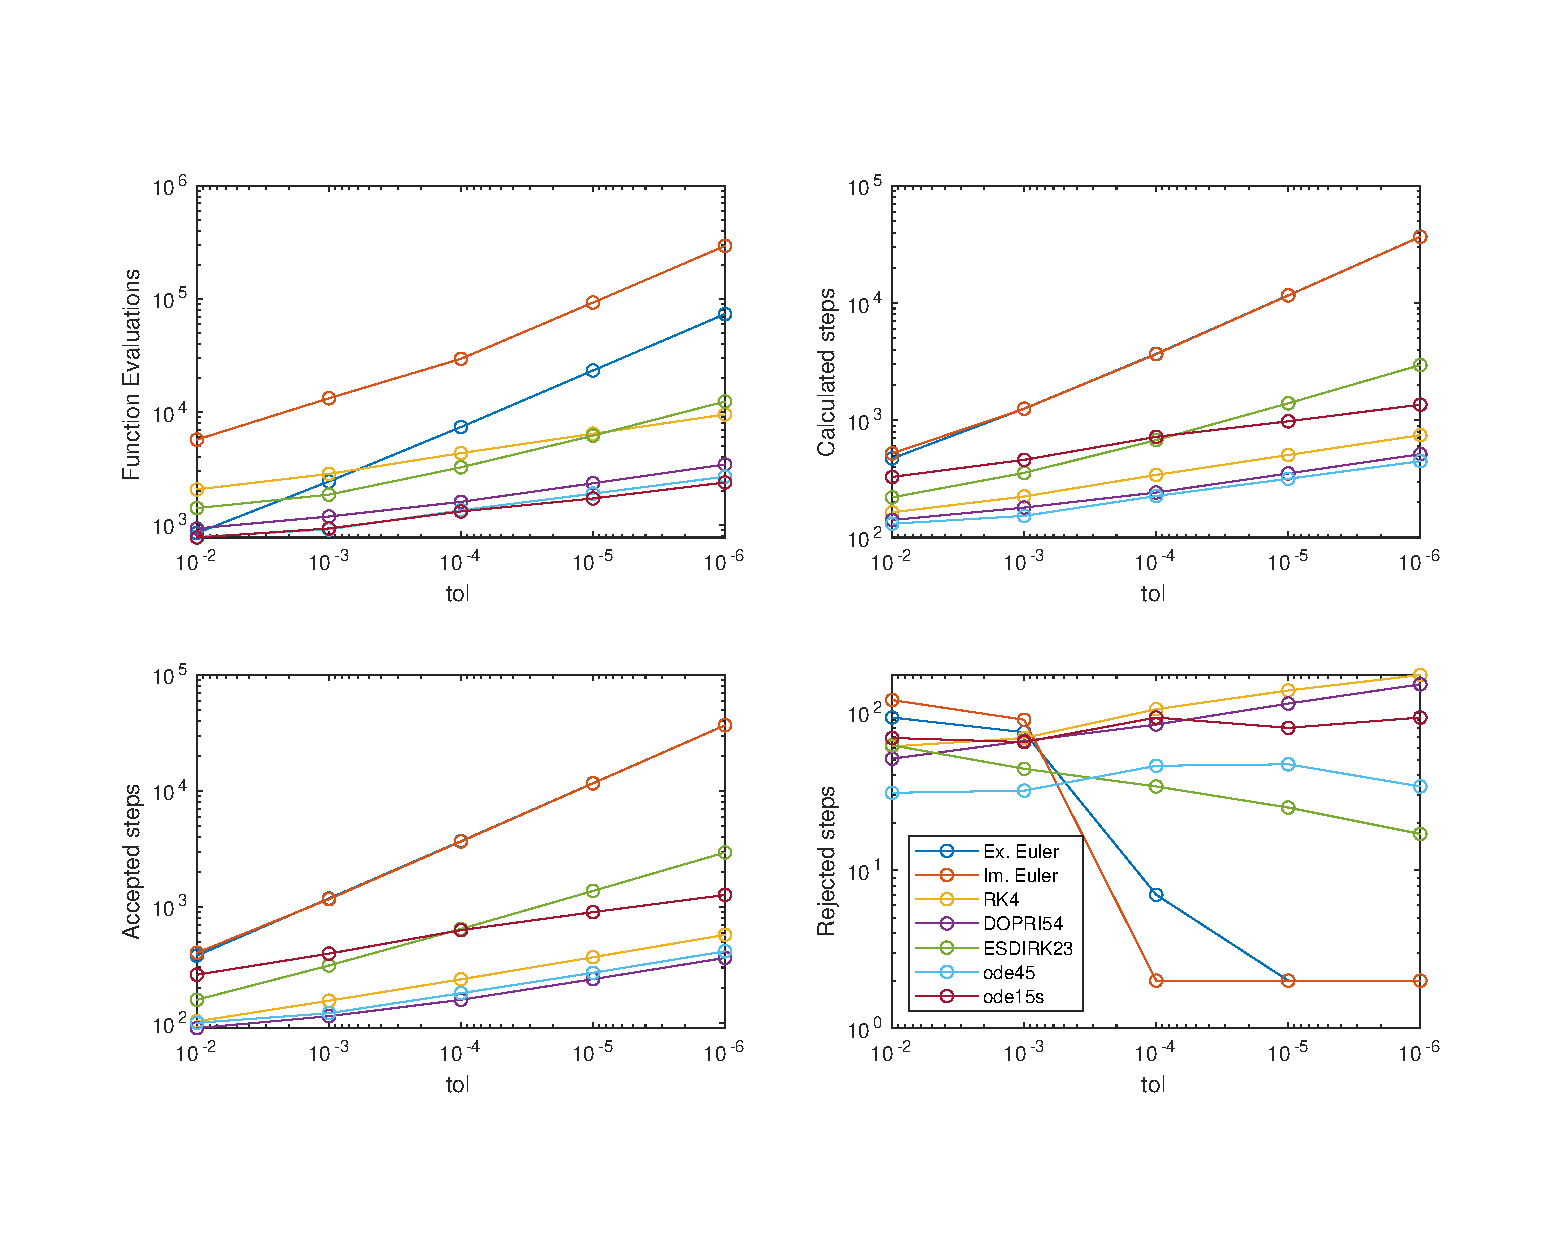
\includegraphics[width=1.25\textwidth]{images/9/9_mu_1_5.pdf}}
    \caption{Performance comparison for the Van der Pol problem ($\mathit{\mu = 1.5}$)}
    \label{9_mu_1_5}
\end{figure}

\begin{figure}[H]
    \centering
    \makebox[\textwidth][c]{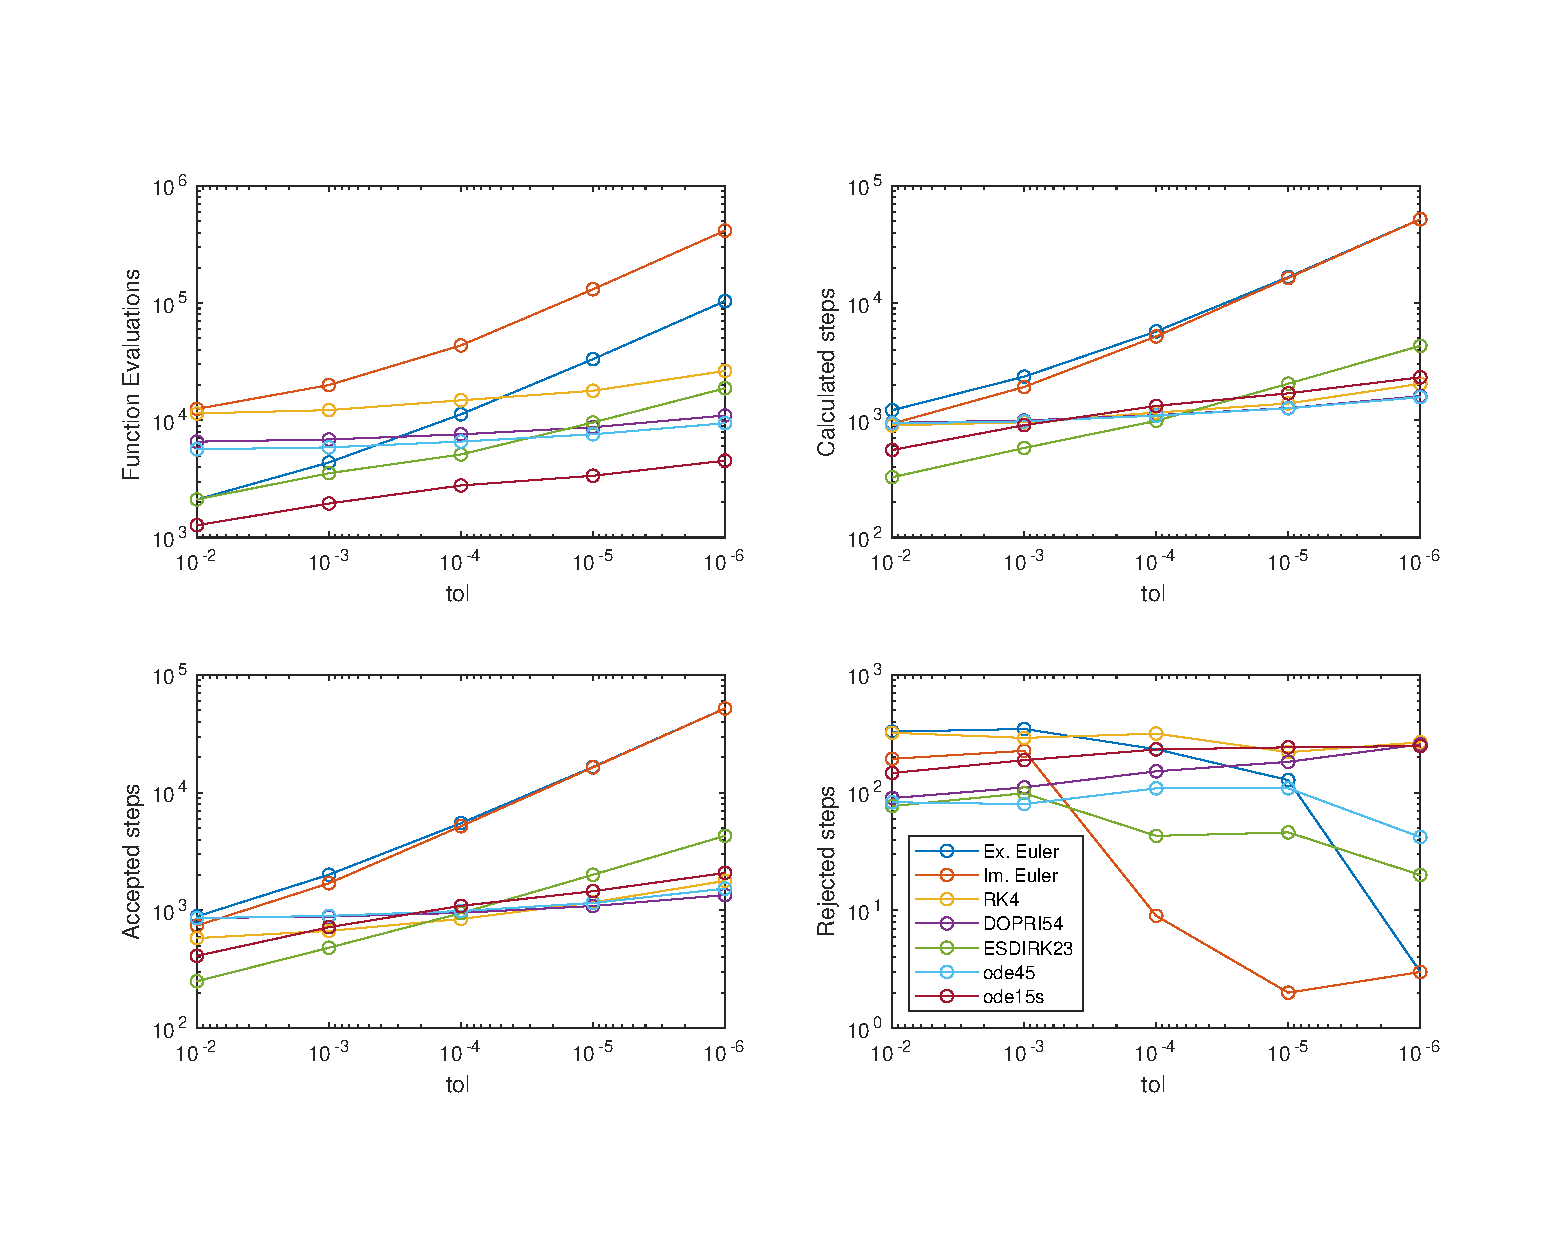
\includegraphics[width=1.25\textwidth]{images/9/9_mu_15.pdf}}
    \caption{Performance comparison for the Van der Pol problem ($\mathit{\mu = 15}$)}
    \label{9_mu_15}
\end{figure}

\begin{figure}[H]
    \centering
    \makebox[\textwidth][c]{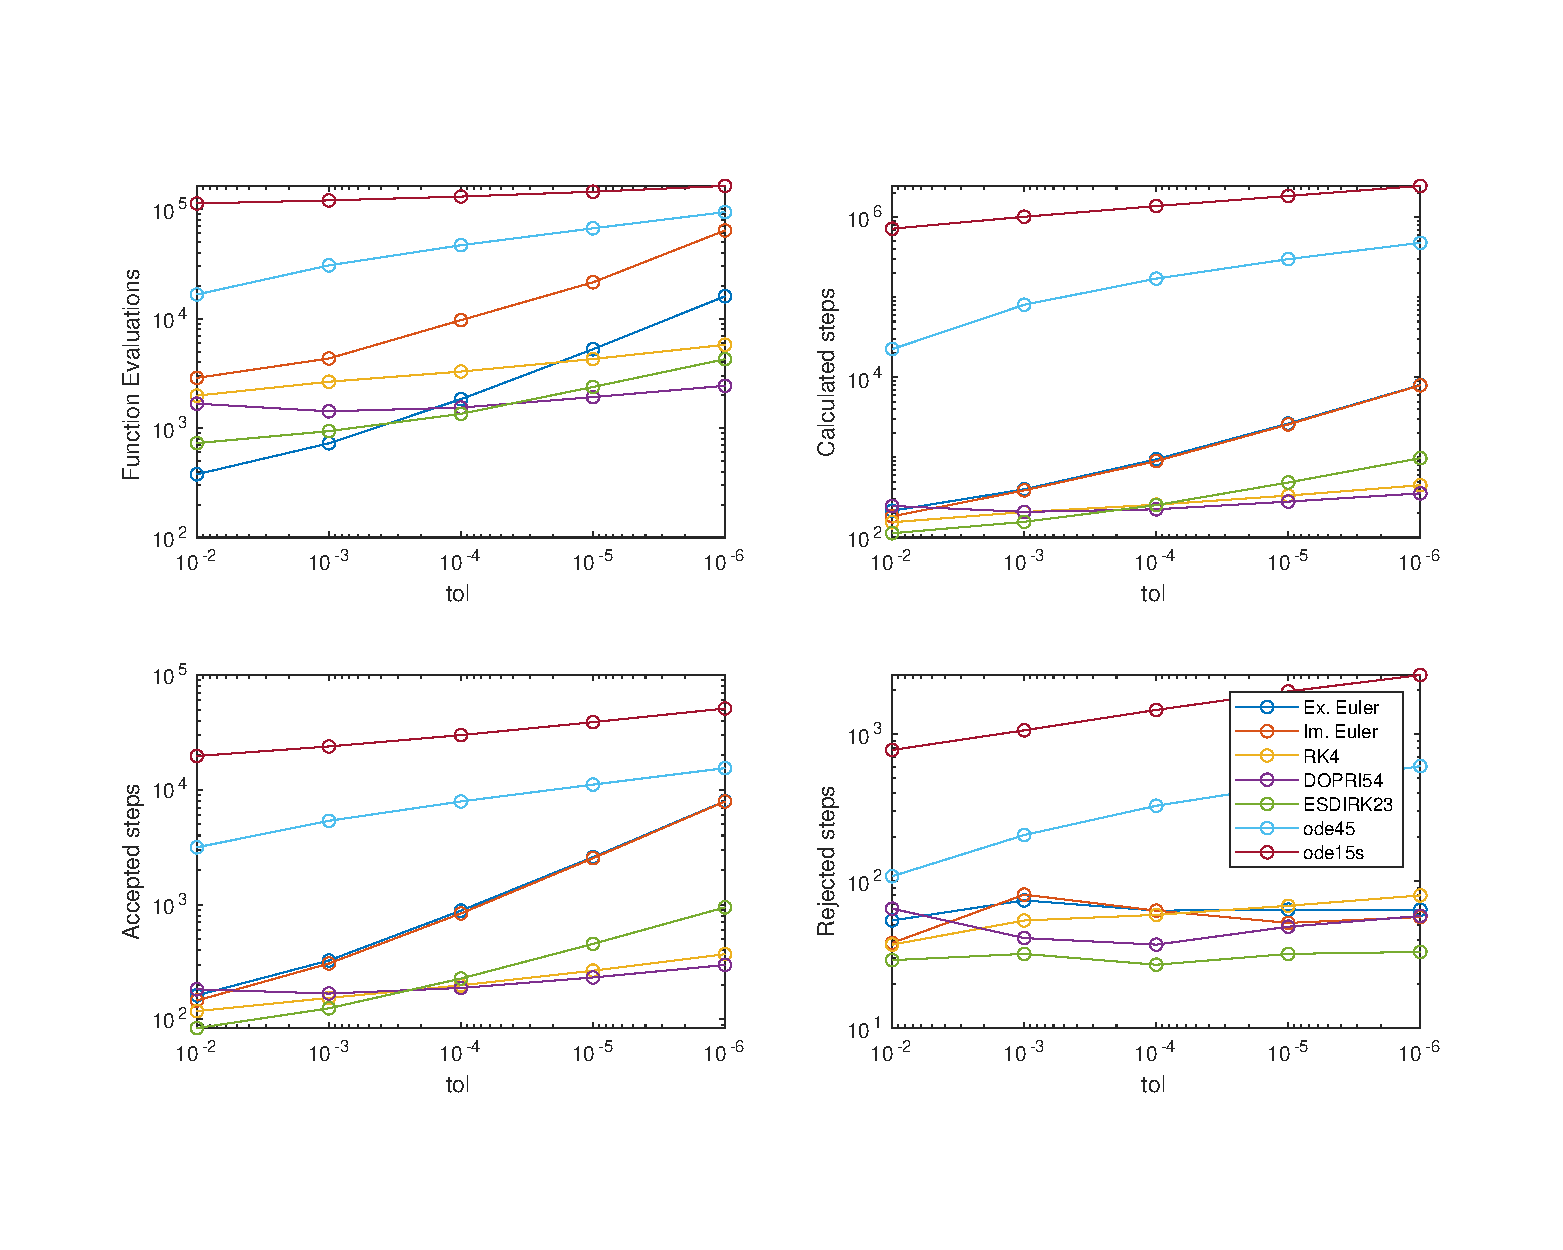
\includegraphics[width=1.25\textwidth]{images/9/9_3D.pdf}}
    \caption{Performance comparison for the CSTR-3D problem}
    \label{9_3D}
\end{figure}

\begin{figure}[H]
    \centering
    \makebox[\textwidth][c]{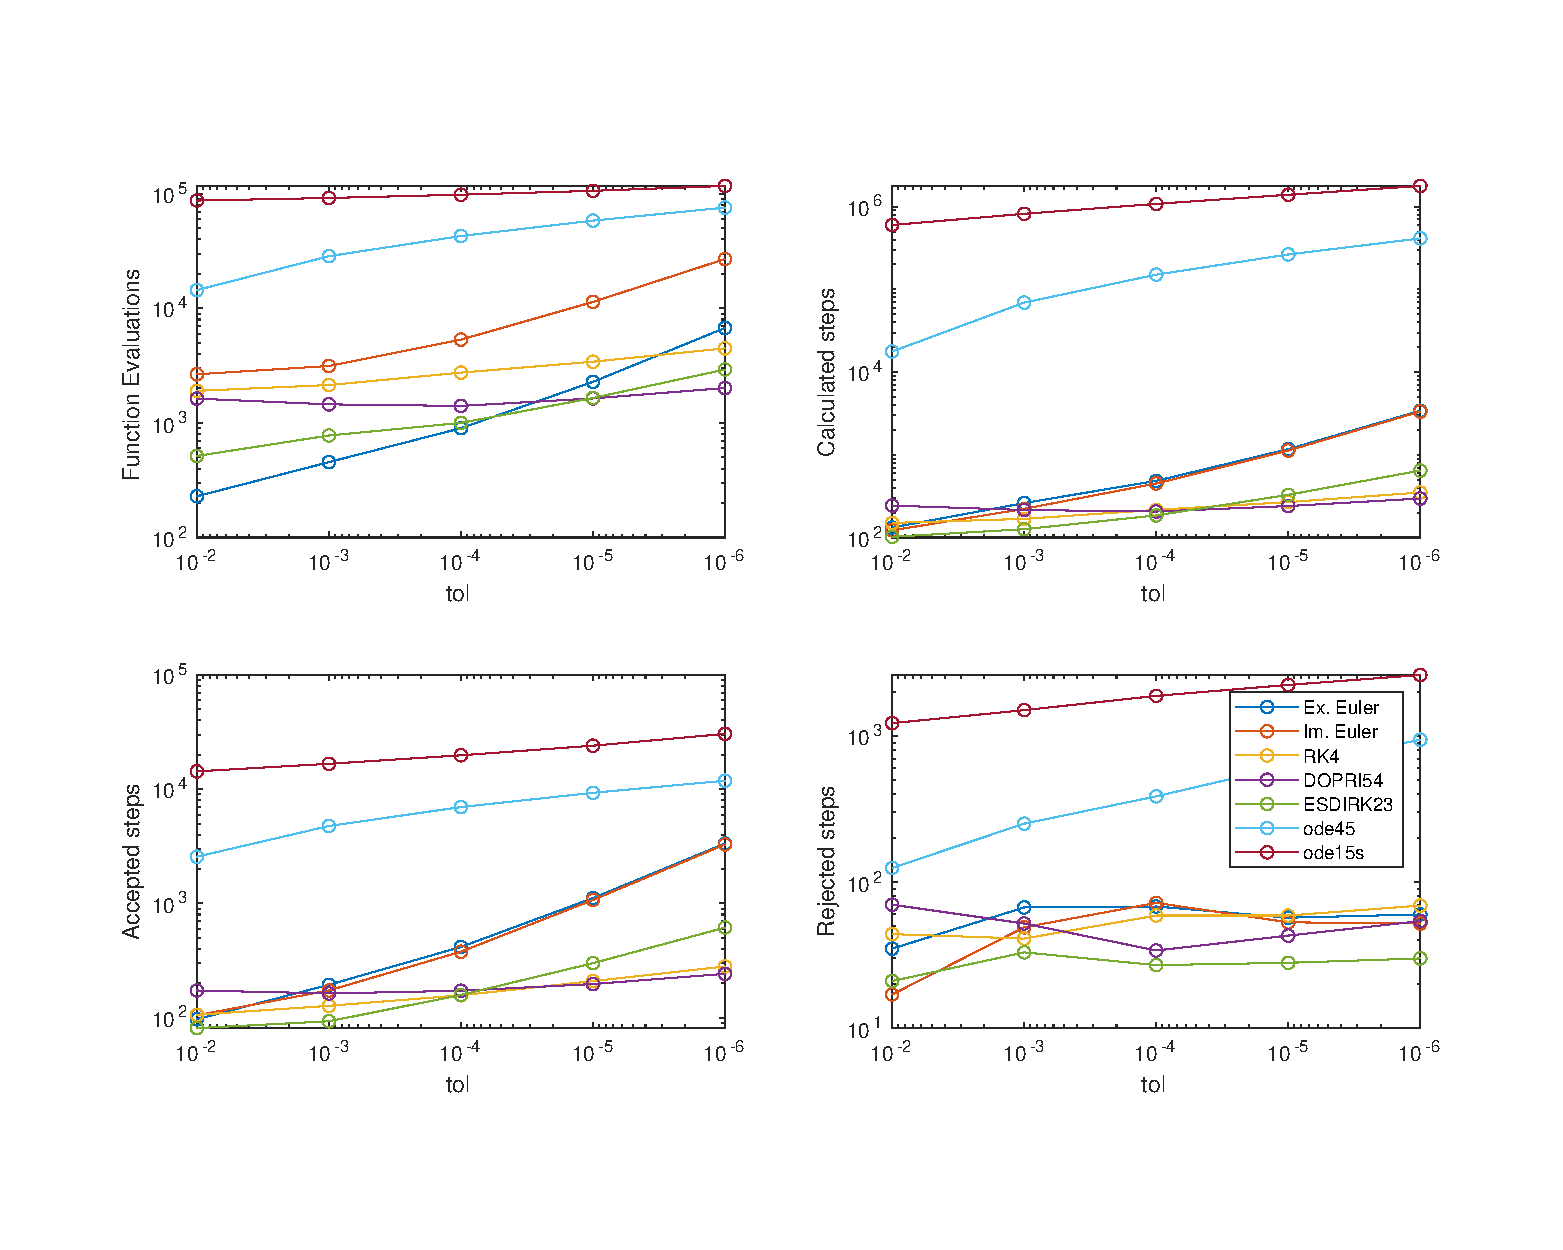
\includegraphics[width=1.25\textwidth]{images/9/9_1D.pdf}}
    \caption{Performance comparison for the CSTR-1D problem }
    \label{9_1D}
\end{figure}